%*****************************************
\chapter{Lambdapi}\label{ch:intro-lambdapi}
%*****************************************

\section{An assembly for proof assistant}

\begin{figure}[t]%[H]
    \centering
    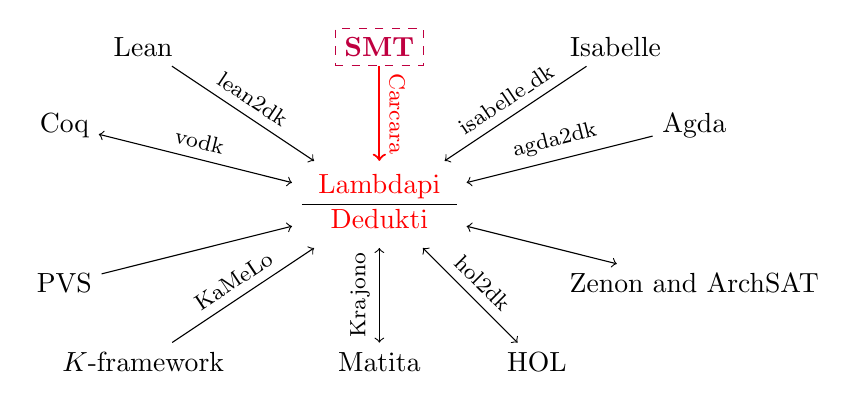
\begin{tikzpicture}
      \path (0,0) node (lp) {\begin{tabular}{c}
        \textcolor{red}{Lambdapi} \\
        \hline
        \textcolor{red}{Dedukti}
      \end{tabular}}
            (-4,1) node (coq) {Coq}
            (-3,2) node (lean) {Lean}
            (0,2) node [draw, dashed, purple] (smt) {\color{purple}\textbf{SMT}}
            (3,2) node (isa) {Isabelle}
            (4,1) node (agda) {Agda}
            (-3,-2) node (k) {$\mathbb{K}$-framework}
            (0,-2) node (mat) {Matita}
            (2,-2) node (hol) {HOL}
            (-4,-1) node (pvs) {PVS}
            (4,-1) node (ze) {Zenon and ArchSAT}
            ;
      \draw[->,red, thick] (smt) -- (lp) node[midway,sloped,above]
      {\footnotesize{Carcara}};
      \draw[->] (lean) -- (lp) node[midway,sloped,above] {\footnotesize{lean2dk}};
      \draw[->] (isa) -- (lp) node[midway,sloped,above] {\footnotesize{isabelle\_dk}};
      \draw[->] (agda) -- (lp) node[midway,sloped,above] {\footnotesize{agda2dk}};
      \draw[<->] (ze) -- (lp) node[midway,sloped,above] {};
      \draw[<->] (hol) -- (lp) node[midway,sloped,above] {\footnotesize{hol2dk}};
      \draw[<->] (mat) -- (lp) node[midway,sloped,above] {\footnotesize{Krajono}};
      \draw[->] (pvs) -- (lp);
      \draw[->] (k) -- (lp) node[midway,sloped,above] {\footnotesize{KaMeLo}};
      \draw[<->] (coq) -- (lp)  node[midway,sloped,above] {\footnotesize{vodk}};
    \end{tikzpicture}
    \caption{Lambdapi, an assembly language for proof systems.}
    \label{fig:interop}
\end{figure}


\section{Typing system}
\label{sect:lambdapi}

Lambdapi is an implementation of $\lambda\Pi$ modulo theory ($\lpm$) \cite{lambdapi}, an extension of the Edinburgh Logical Framework $\lambda\Pi$ \cite{lf}, a simply typed $\lambda$-calculus with dependent types. $\lpm$ adds user-defined higher-order rewrite rules. Its syntax is given by
%
\begin{align*}
&\text{Universes}  &u &::= \index{\type} ~|~ \index{\kind} \\
&\text{Terms}   &t,v, A,B,C &::= c ~|~ x ~|~ u ~|~ \Pi\,x : A,\,B~|~ \lambda\,x : A,\,t ~|~t~v \\
&\text{Contexts}   &\Gamma &::= \langle \rangle ~|~ \Gamma, x : A \\
&\text{Signatures}  &\Sigma &::= \langle \rangle ~|~ \Sigma, c : C ~|~ \Sigma, c := t : C ~|~ \Sigma, t \hookrightarrow v 
\end{align*}
%
where $c$ is a constant and $x$ is a variable  (ranging over disjoint sets), $C$ is a closed term. \emph{Universes} are constants used to verify if a type is well-formed -- more details can be found in \cite[\S 2.1]{lf}. $\Pi\,x : A.\,B$ is the dependent product, and we write $A \rightarrow B$ when $x$ does not appear free in $B$, $\lambda\,x : A.\,t$ is an abstraction, and  $t~v$ is an application.
A \emph{(local) context} \index{$\Gamma$} is a finite sequence of variable declarations $x:A$ introducing variables and their types.
A \emph{signature} \index{$\Sigma$} representing the global context is a finite sequence of \emph{assumptions} $c : C$, indicating that constant $c$ is of type $C$, \emph{definitions} $c := t : C$, indicating that $c$ has the value $t$ and type $C$, and \emph{rewrite rules} $t \hookrightarrow v$ such that $t = c~v_1 \dots v_n$ where $c$ is a constant.

The relation $\hookrightarrow_{\beta\Sigma}$ is generated by $\beta$-reduction and by the rewrite rules of $\Sigma$. The relation $\hookrightarrow_{\beta\Sigma}^*$ denotes the reflexive and transitive closure of $\hookrightarrow_{\beta\Sigma}$, and the relation $\equiv_{\beta\Sigma}$ (called \emph{conversion}) the reflexive, symmetric, and transitive closure of $\hookrightarrow_{\beta\Sigma}$. 
The relation $\hookrightarrow_{\beta\Sigma}$ must be confluent, i.e.,
whenever $t \hookrightarrow_{\beta\Sigma}^* v_1$ and $t \hookrightarrow_{\beta\Sigma}^* v_2$, there exists a term $w$ such that $v_1 \hookrightarrow_{\beta\Sigma}^* w$ and $v_2 \hookrightarrow_{\beta\Sigma}^* w$, and it must preserve typing, i.e., 
whenever $\Gamma \vdash_\Sigma t: A$ and $t \hookrightarrow_{\beta\Sigma} v$ then $\Gamma \vdash_\Sigma v: A$ \cite{blanqui:LIPIcs.FSCD.2020.13}.

A Lambdapi typing judgment $\Gamma \vdash_\Sigma t : A$ asserts that term $t$ has type $A$ in the context $\Gamma$ and the signature $\Sigma$.
The typing rules, shown in \cref{fig:lp-typing-rules}, are similar to those of  $\lambda\Pi$ \cite[\S 2]{lf}, except for the additional rule (Conv) that identifies types modulo~\index{$\equiv_{\beta\Sigma}$} instead of just modulo $\beta$-reduction. 


\begin{figure}
  \[
    \begin{prooftree}
      \infer0[(Empty)]{ \vdash_\Sigma \langle\,\rangle  }
    \end{prooftree}
    \qquad
    \begin{prooftree}
      \hypo{ \vdash_\Sigma \Gamma }
      \hypo{ \Gamma \vdash_\Sigma A : s }
      \infer2[(Decl) $x \notin \Gamma$]{ \vdash_\Sigma \Gamma, x : A  }
    \end{prooftree}
  \]
  \medskip
  \begin{center}
    \begin{prooftree}
    \hypo{ \vdash_\Sigma \Gamma }
    \hypo{\Gamma \vdash_\Sigma A : s}
    \infer2[(Const)]{ \Gamma \vdash_\Sigma c : A }
    \end{prooftree}
  \end{center}
  \medskip
  \[
    \begin{prooftree}
      \hypo{ \vdash_\Sigma \Gamma } 
      \infer1[(Sort)]{ \Gamma \vdash_\Sigma \type : \kind }
    \end{prooftree}
    \qquad
    \begin{prooftree}
      \hypo{ \vdash_\Sigma \Gamma }
      \infer1[(Var) $x : A \in \Sigma$]{ \Gamma \vdash_\Sigma x : A }
    \end{prooftree}
  \]
  \medskip
  \begin{center}
    \begin{prooftree}
    \hypo{\Gamma, \vdash_\Sigma A : \type }
    \hypo{\Gamma, x: A \vdash_\Sigma B: s}
    \hypo{\Gamma, x : A \vdash_\Sigma t: B}
    \infer3[(Abs)]{ \Gamma \vdash_\Sigma \lambda x: A, t : \Pi x : A, B }
    \end{prooftree}
  \end{center}
  
  \[
    \begin{prooftree}
      \hypo{ \Gamma \vdash_\Sigma A : \type } 
      \hypo{ \Gamma, x : A \vdash_\Sigma B : s } 
      \infer2[(Prod)]{ \Gamma \vdash_\Sigma \Pi x : A, B : s }
    \end{prooftree}
    \quad
    \begin{prooftree}
      \hypo{ \Gamma \vdash t : \Pi x : A, B }
      \hypo{ \Gamma \vdash  u : A }
      \infer2[(App)]{ \Gamma \vdash_\Sigma t~u : B[u \leftarrow x] }
    \end{prooftree}
  \]
  \begin{center}
  \begin{prooftree}
  \hypo{\Gamma, \vdash_\Sigma B: u}
  \hypo{\Gamma \vdash_\Sigma t: A}
  \hypo{A \equiv_{\beta\Sigma} B}
  \infer3[(Conv)]{ \Gamma \vdash_\Sigma t: B }
  \end{prooftree}
  \end{center}
  \caption{Typing rules of $\lpm$}
  \label{fig:lp-typing-rules}
  \end{figure}
